\documentclass[12pt]{standalone}

\usepackage{tikz}
\usepackage{ctex}

\tikzset{steiner/.style={color=red}}
\tikzset{tree node/.style={circle,draw}}

\begin{document}
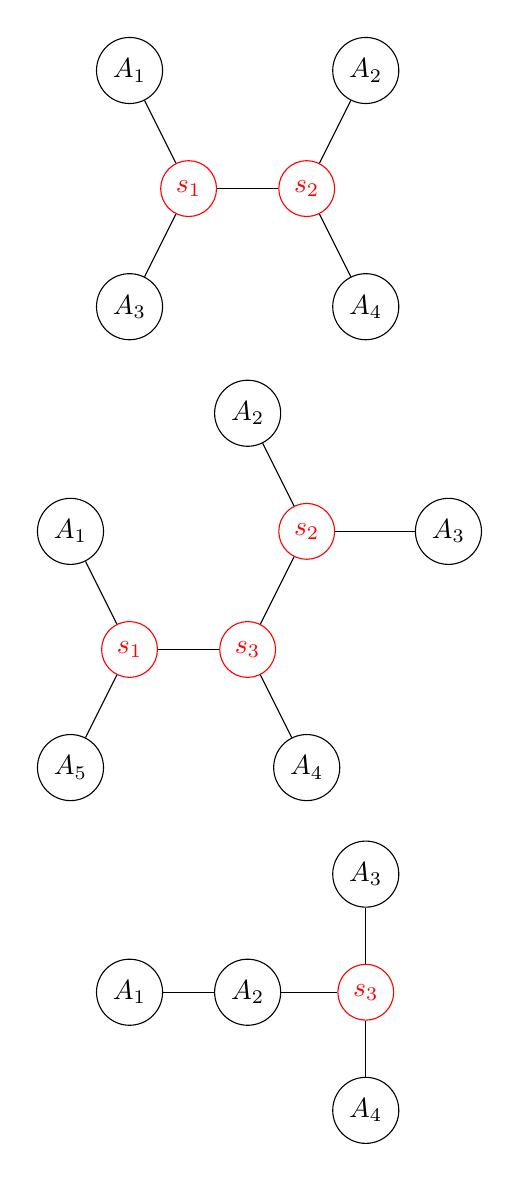
\begin{tikzpicture}[x=1.5cm,y=1.5cm]

\matrix[row sep=5mm] {
    % tree 1
    \node (A1) [tree node] at (0,1) {$A_1$};
    \node (A2) [tree node] at (2,1) {$A_2$};
    \node (A3) [tree node] at (0,-1) {$A_3$};
    \node (A4) [tree node] at (2,-1) {$A_4$};
    \node (S1) [tree node,steiner] at (0.5,0) {$s_1$};
    \node (S2) [tree node,steiner] at (1.5,0) {$s_2$};

    \draw (S1) -- (A1);
    \draw (S1) -- (A3);
    \draw (S2) -- (A2);
    \draw (S2) -- (A4);
    \draw (S1) -- (S2);
    \\
    % tree 2
    \node (A1) [tree node] at (-0.5,1) {$A_1$};
    \node (A2) [tree node] at (1,2) {$A_2$};
    \node (A3) [tree node] at (2.7,1) {$A_3$};
    \node (A4) [tree node] at (1.5,-1) {$A_4$};
    \node (A5) [tree node] at (-0.5,-1) {$A_5$};
    \node (S1) [tree node,steiner] at (0,0) {$s_1$};
    \node (S2) [tree node,steiner] at (1.5,1) {$s_2$};
    \node (S3) [tree node,steiner] at (1,0) {$s_3$};

    \draw (S1) -- (A1);
    \draw (S1) -- (A5);
    \draw (S1) -- (S3);
    \draw (S2) -- (A2);
    \draw (S2) -- (A3);
    \draw (S3) -- (S2);
    \draw (S3) -- (A4);
    \\
    % tree 3
    \node (A1) [tree node] at (0,0) {$A_1$};
    \node (A2) [tree node] at (1,0) {$A_2$};
    \node (A3) [tree node] at (2,1) {$A_3$};
    \node (A4) [tree node] at (2,-1) {$A_4$};
    \node (S3) [tree node,steiner] at (2,0) {$s_3$};

    \draw (A1) -- (A2);
    \draw (A2) -- (S3);
    \draw (S3) -- (A3);
    \draw (S3) -- (A4);
    \\
};

\end{tikzpicture}
\end{document}
